\chapter{Appendix}
The code can be found at: \url{https://github.com/MelissaJessen/Shallow-Water-Equations}.


\section{Additional figures from 1D SWE spherical CNN and FNO}
Results for the other sigma values.

CNN, $\sigma = \frac{\pi}{8}$.
\begin{figure}[H]
    \centering
    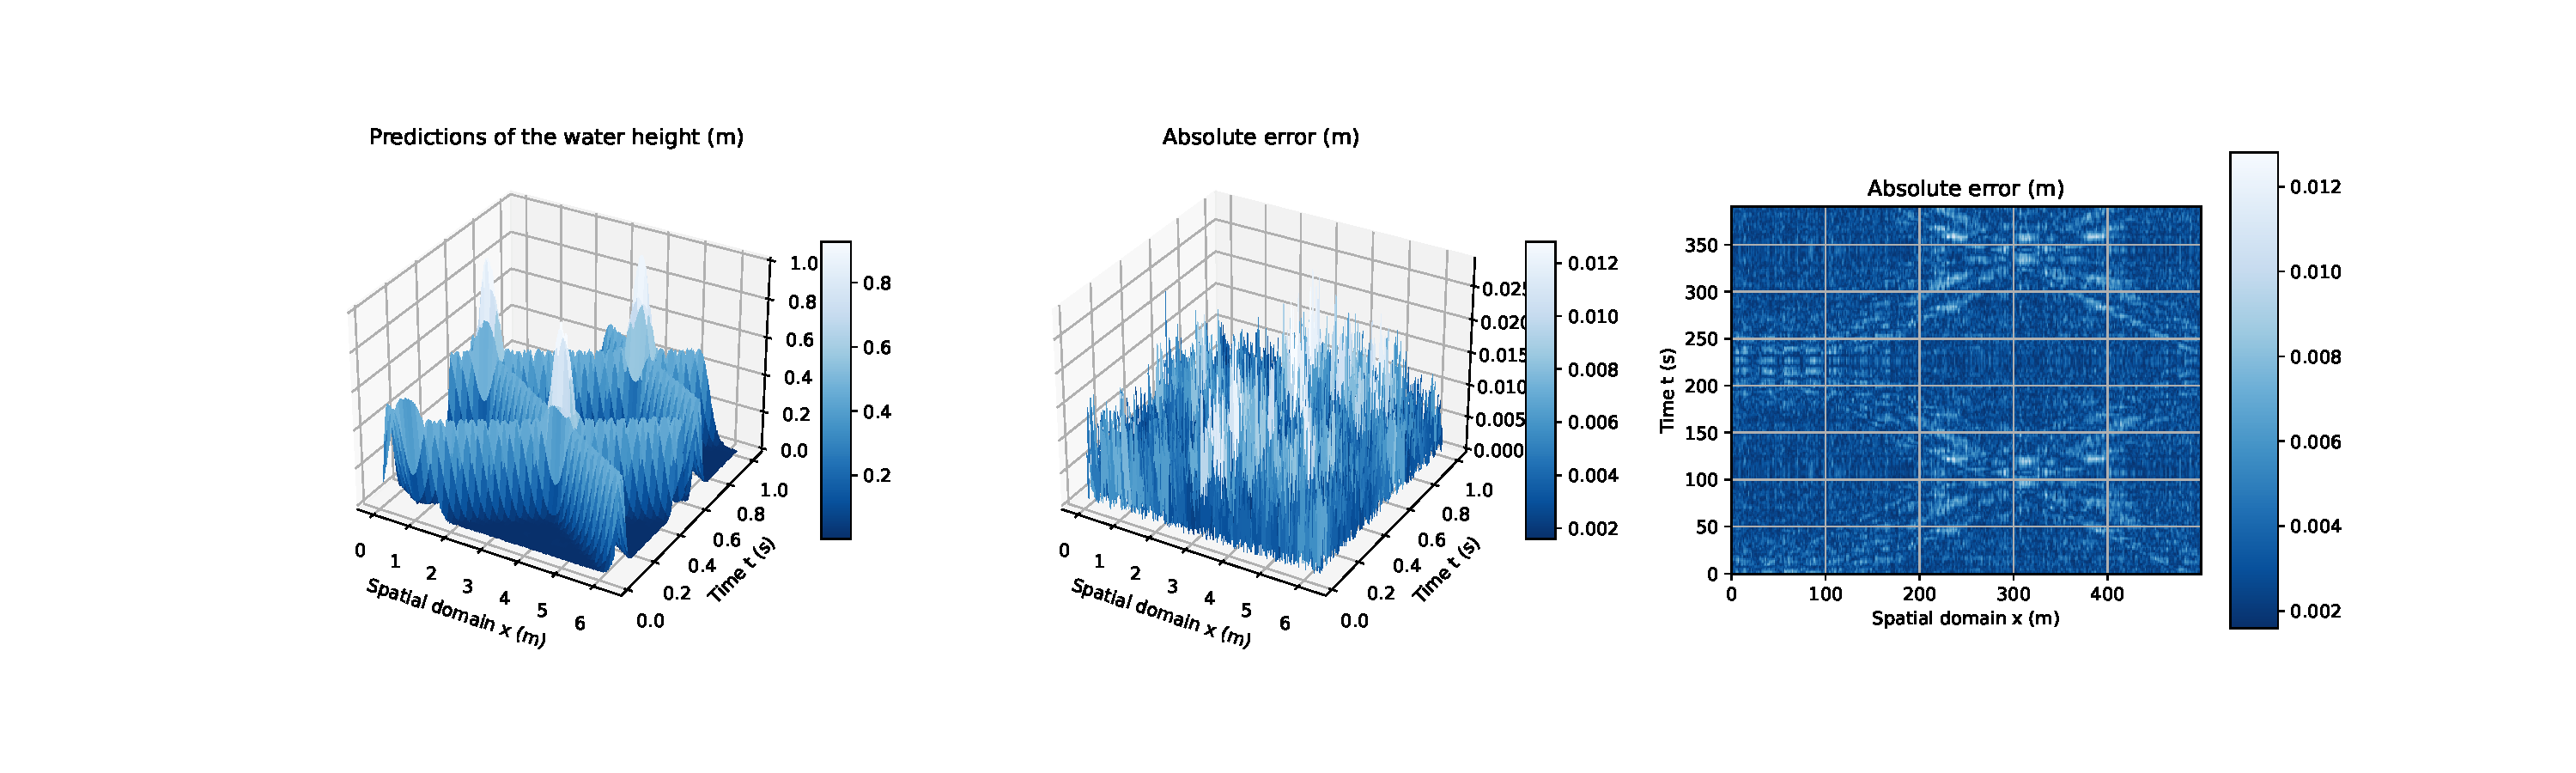
\includegraphics[width=\textwidth]{C:/Users/Matteo/Shallow-Water-Equations/plots/Spherical_linear_1D_CNN_error_sigma=1.pdf}
    \caption{Error for the 1D SWE spherical CNN with sigma=1.}
\end{figure}

\begin{figure}[H]
    \centering
    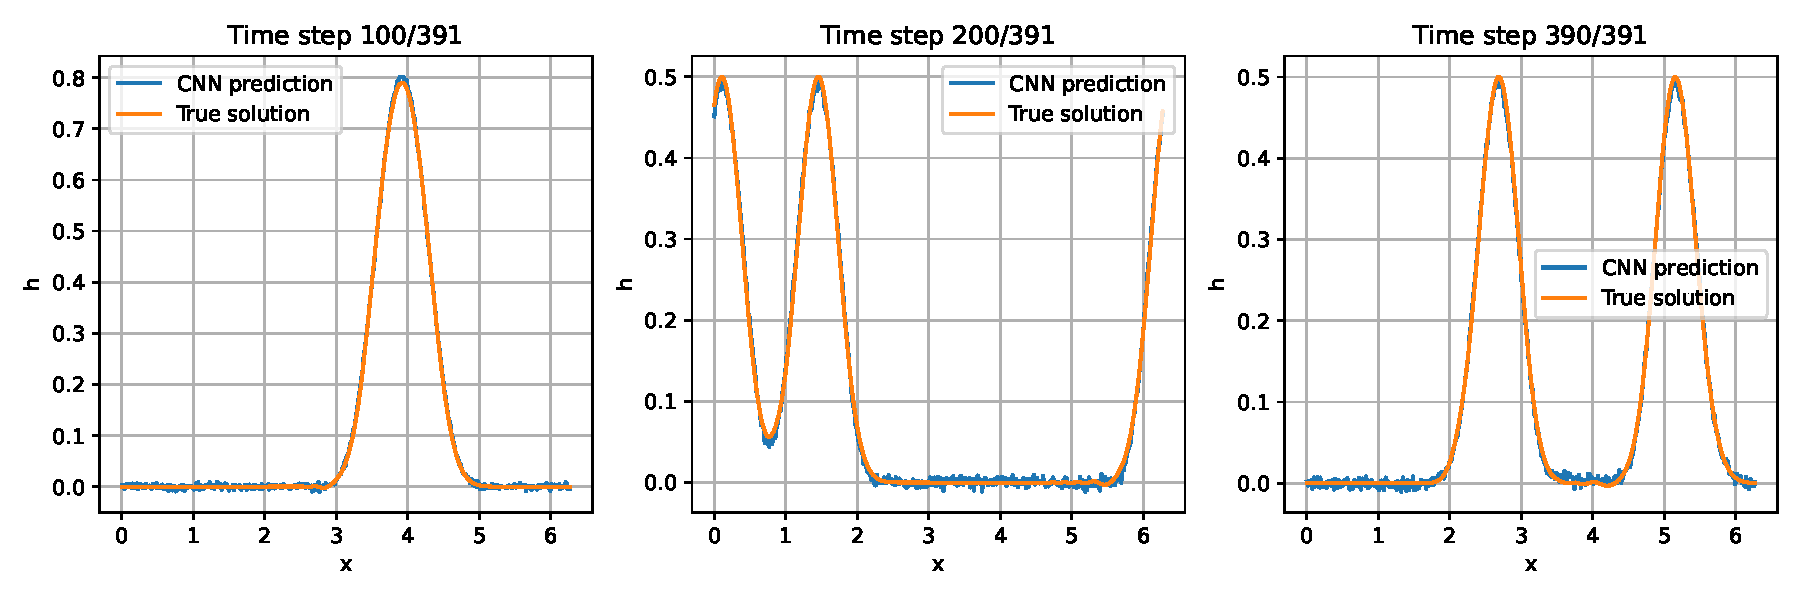
\includegraphics[width=\textwidth]{C:/Users/Matteo/Shallow-Water-Equations/plots/Spherical_linear_1D_CNN_time_steps_sigma=1.pdf}
    \caption{Results for the 1D SWE spherical CNN with sigma=1.}
\end{figure}

CNN $\sigma = \frac{\pi}{32}$.
\begin{figure}[H]
    \centering
    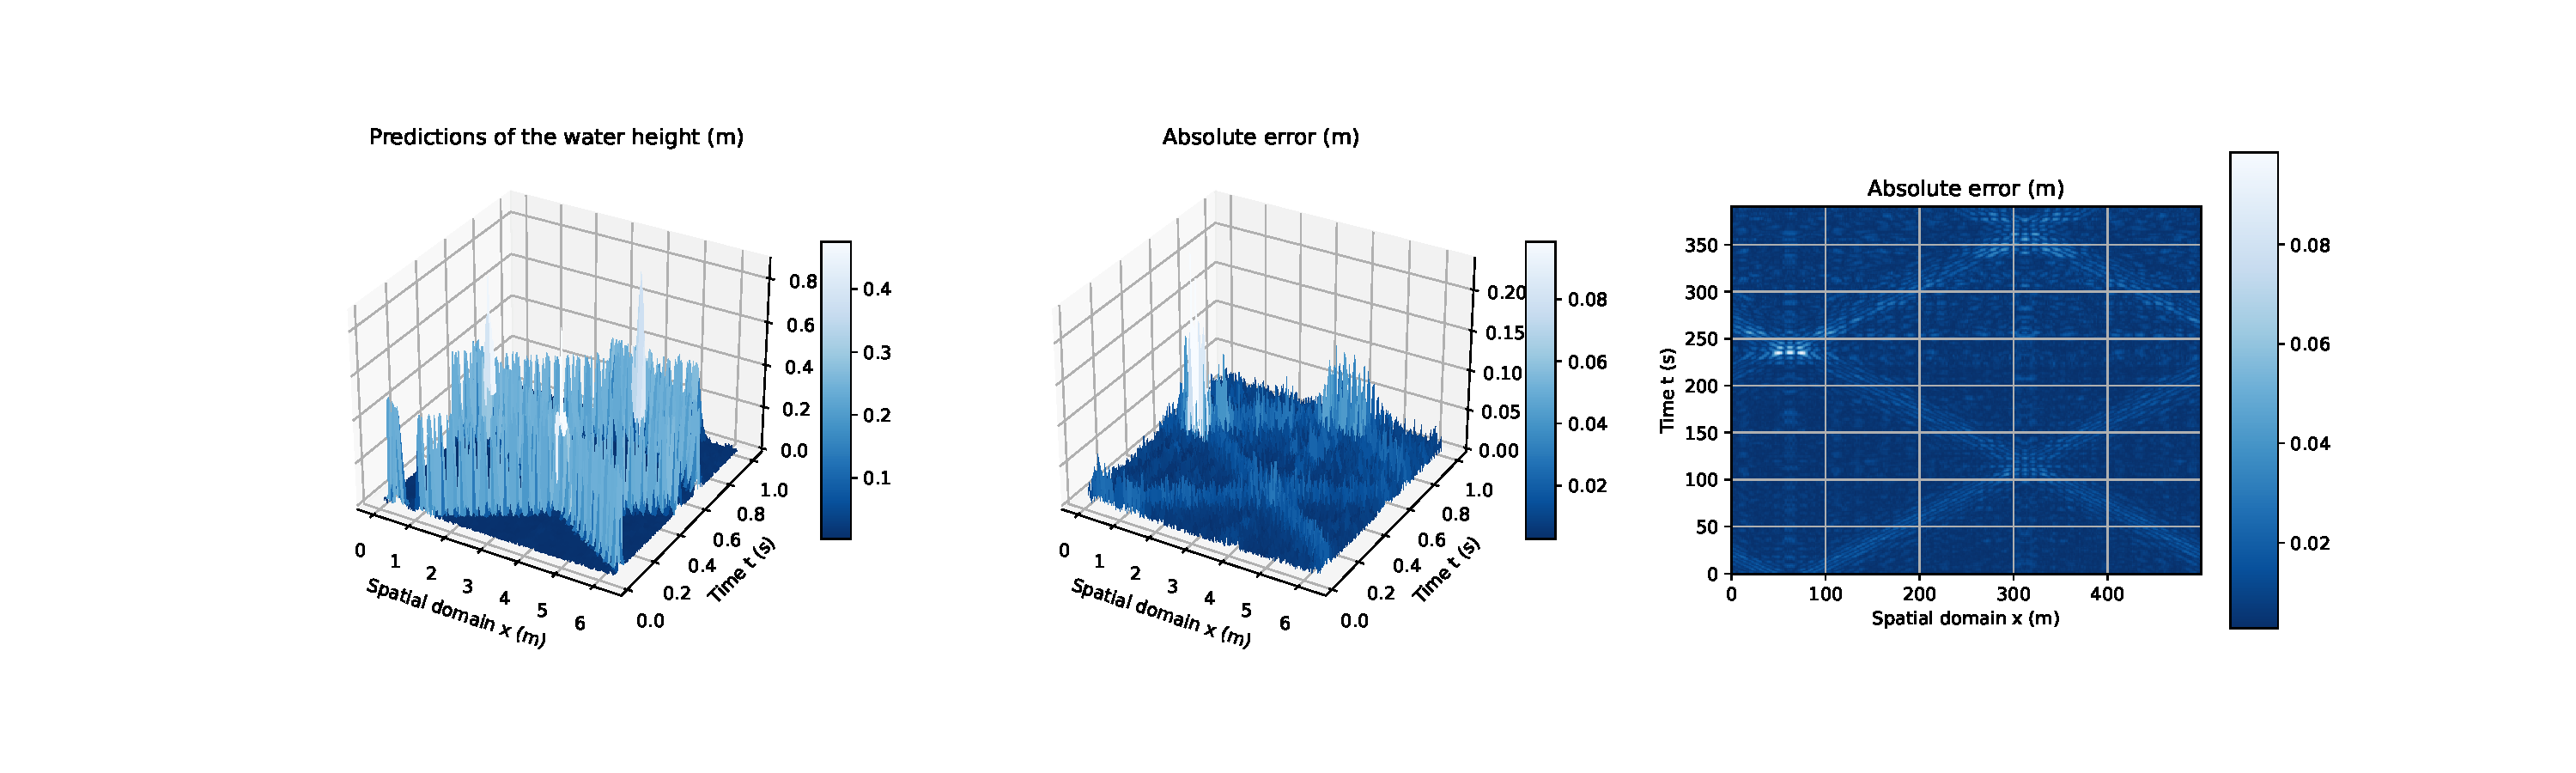
\includegraphics[width=\textwidth]{C:/Users/Matteo/Shallow-Water-Equations/plots/Spherical_linear_1D_CNN_error_sigma=3.pdf}
    \caption{Error for the 1D SWE spherical CNN with sigma=1.}
\end{figure}

\begin{figure}[H]
    \centering
    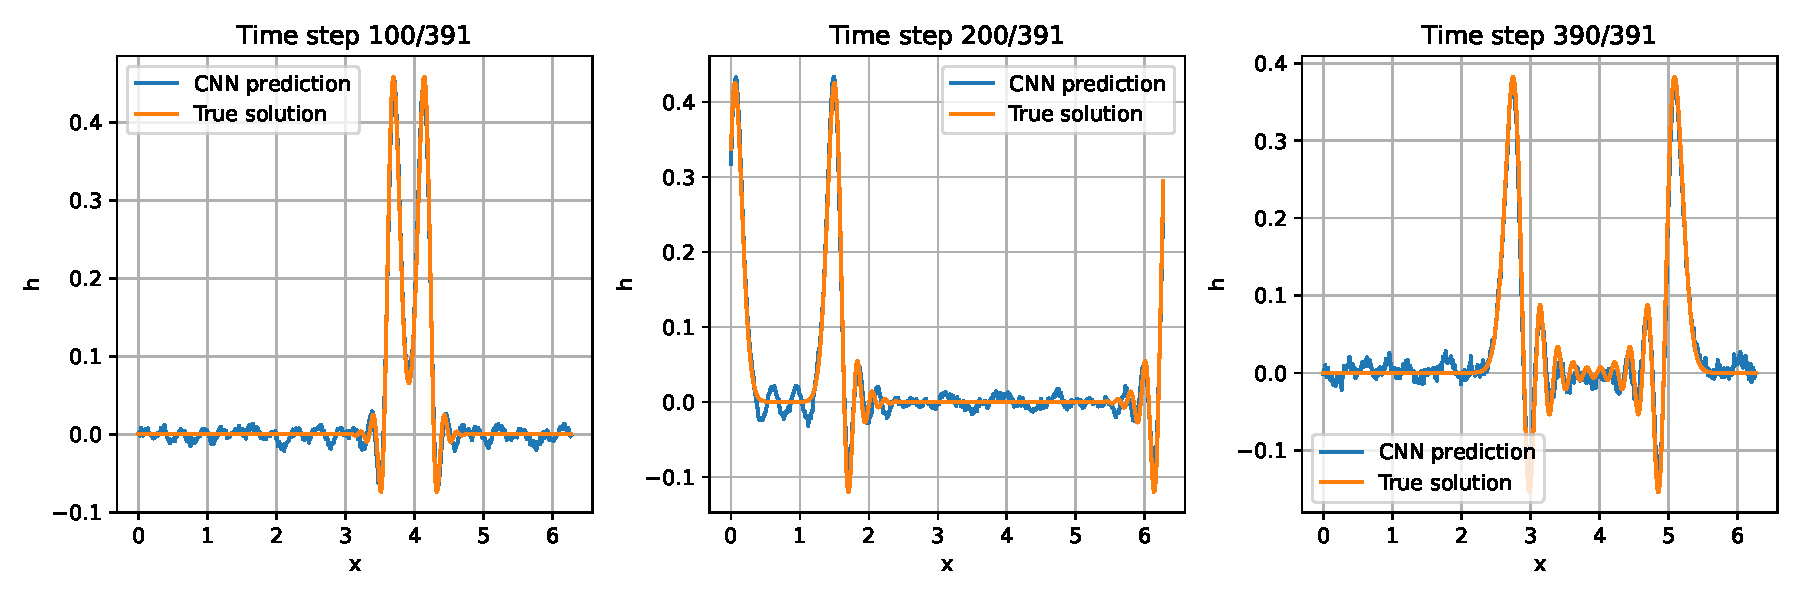
\includegraphics[width=\textwidth]{C:/Users/Matteo/Shallow-Water-Equations/plots/Spherical_linear_1D_CNN_time_steps_sigma=3.pdf}
    \caption{Results for the 1D SWE spherical CNN with sigma=1.}
\end{figure}

FNO, $\sigma = \frac{\pi}{8}$.
\begin{figure}[H]
    \centering
    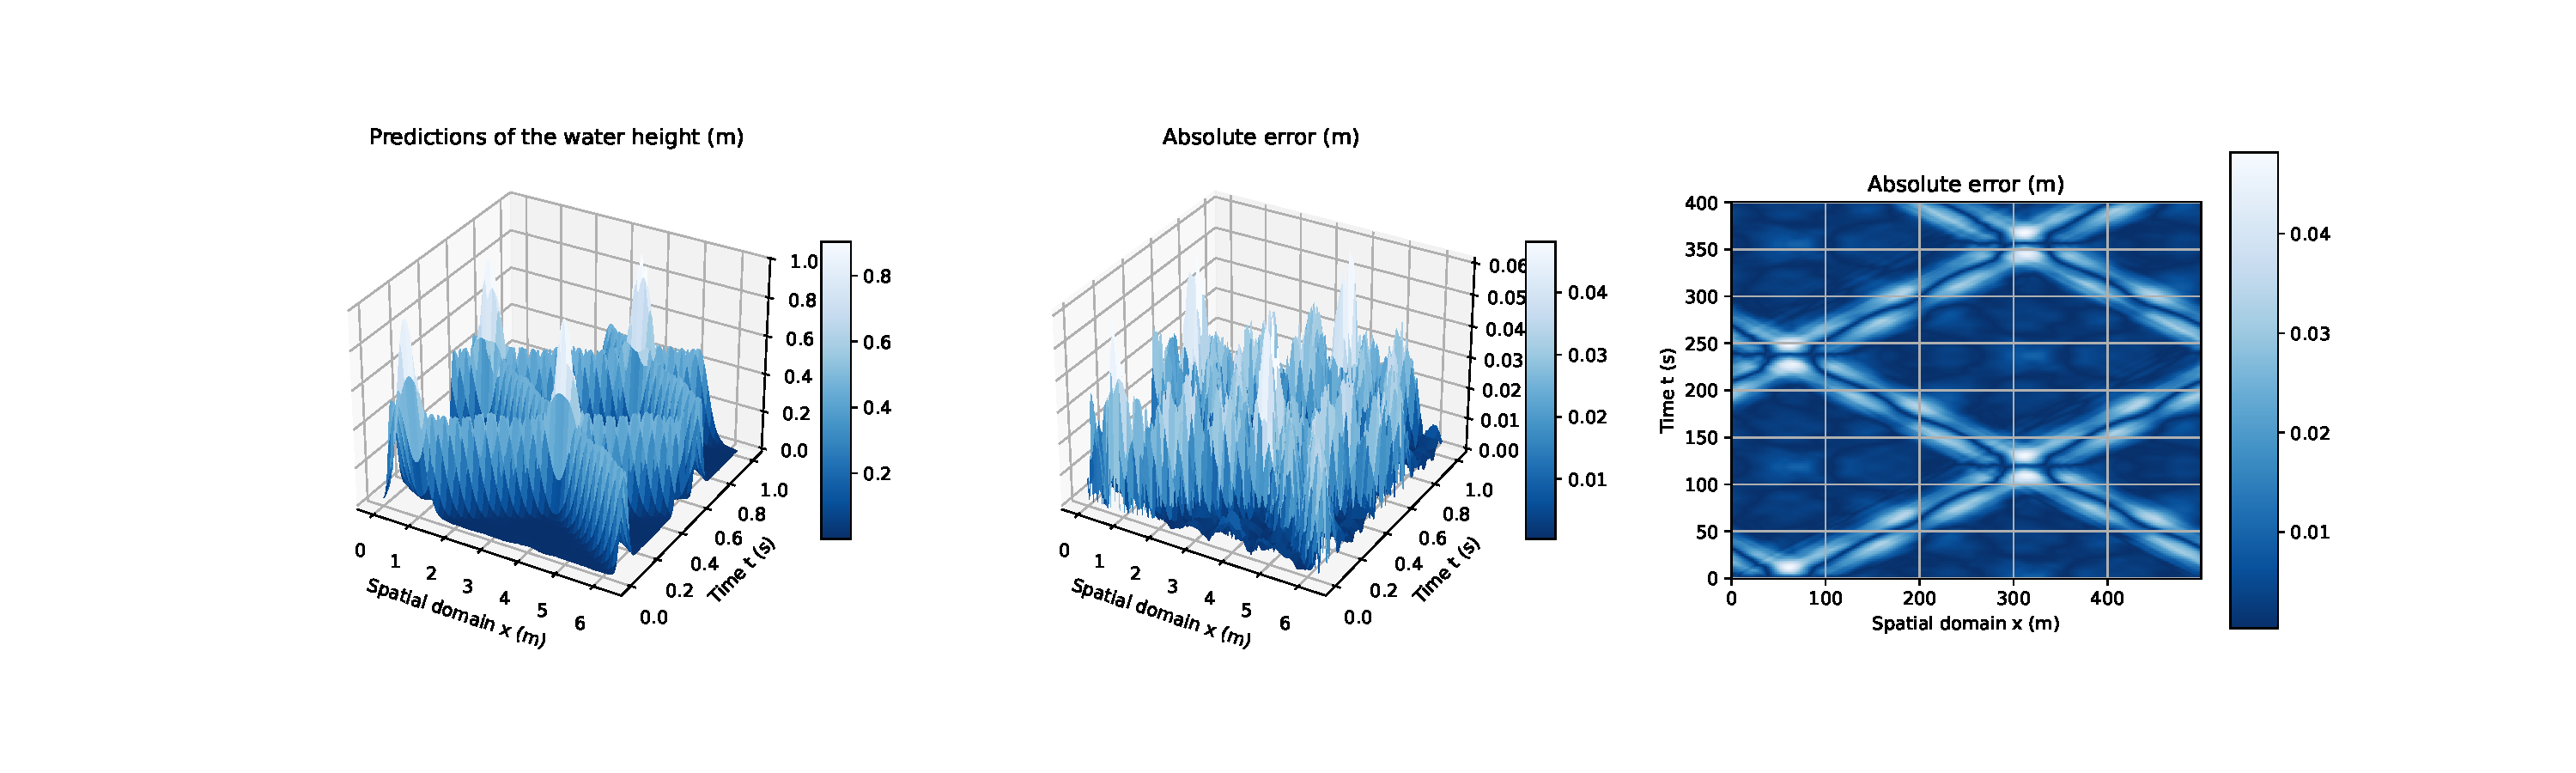
\includegraphics[width=\textwidth]{C:/Users/Matteo/Shallow-Water-Equations/plots/Spherical_linear_1D_FNO_error_sigma=1.pdf}
    \caption{Error for the 1D SWE spherical CNN with sigma=1.}
\end{figure}

\begin{figure}[H]
    \centering
    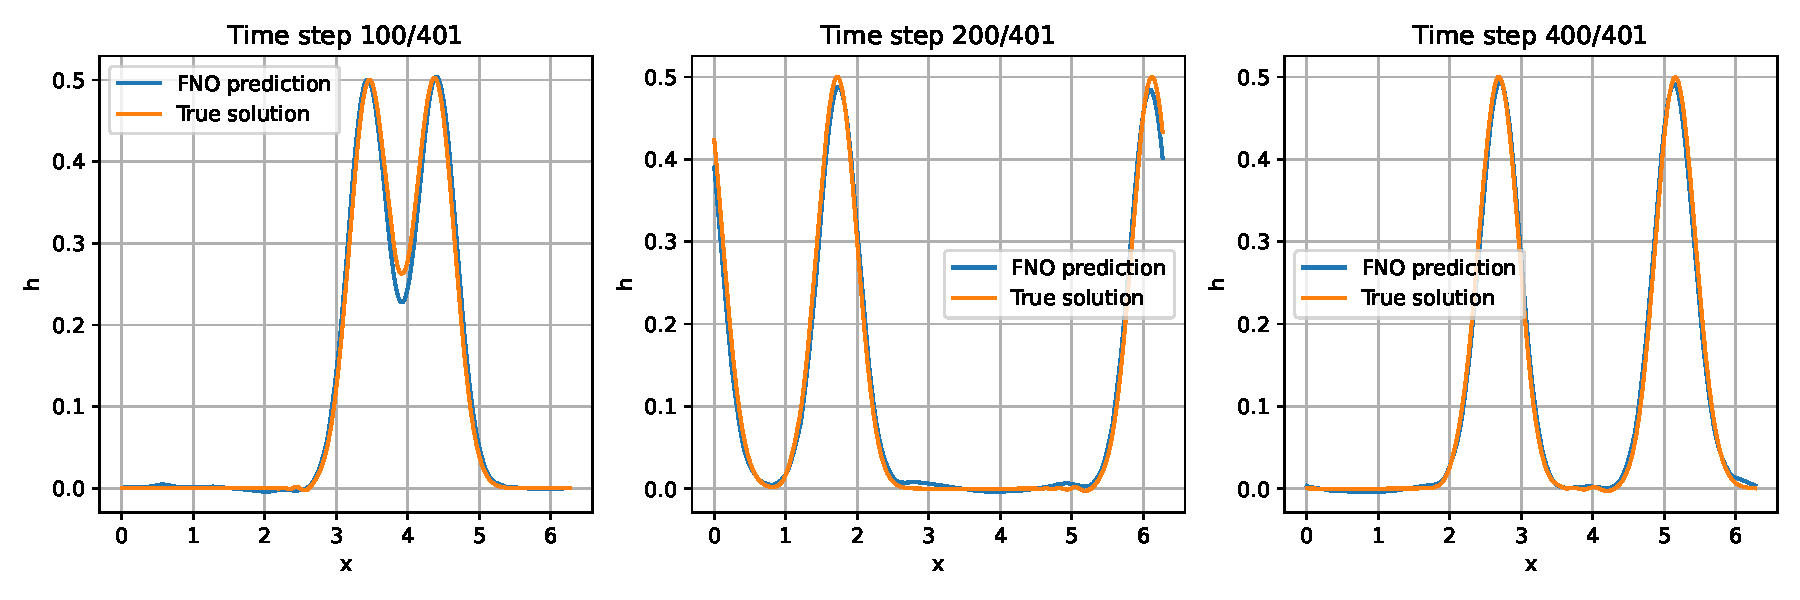
\includegraphics[width=\textwidth]{C:/Users/Matteo/Shallow-Water-Equations/plots/Spherical_linear_1D_FNO_timesteps_sigma=1.pdf}
    \caption{Results for the 1D SWE spherical CNN with sigma=1.}
\end{figure}

FNO $\sigma = \frac{\pi}{32}$.
\begin{figure}[H]
    \centering
    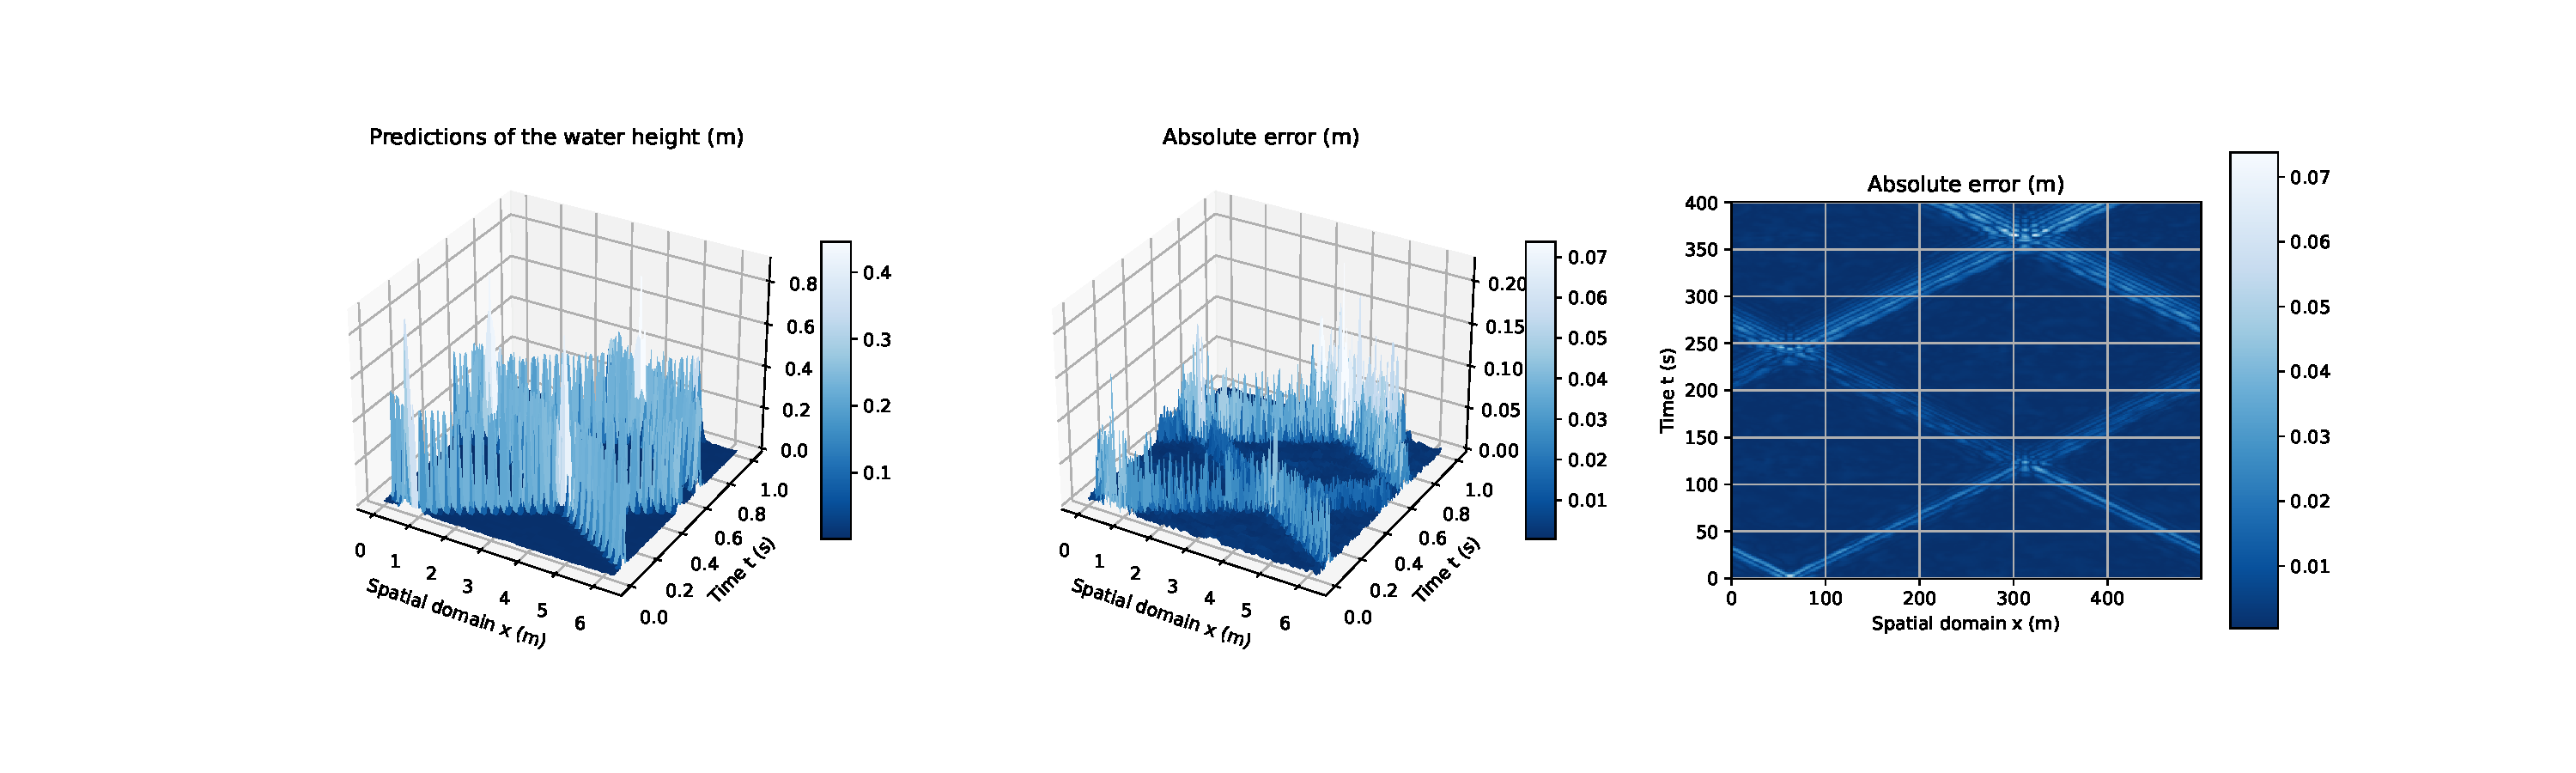
\includegraphics[width=\textwidth]{C:/Users/Matteo/Shallow-Water-Equations/plots/Spherical_linear_1D_FNO_error_sigma=3.pdf}
    \caption{Error for the 1D SWE spherical CNN with sigma=1.}
\end{figure}

\begin{figure}[H]
    \centering
    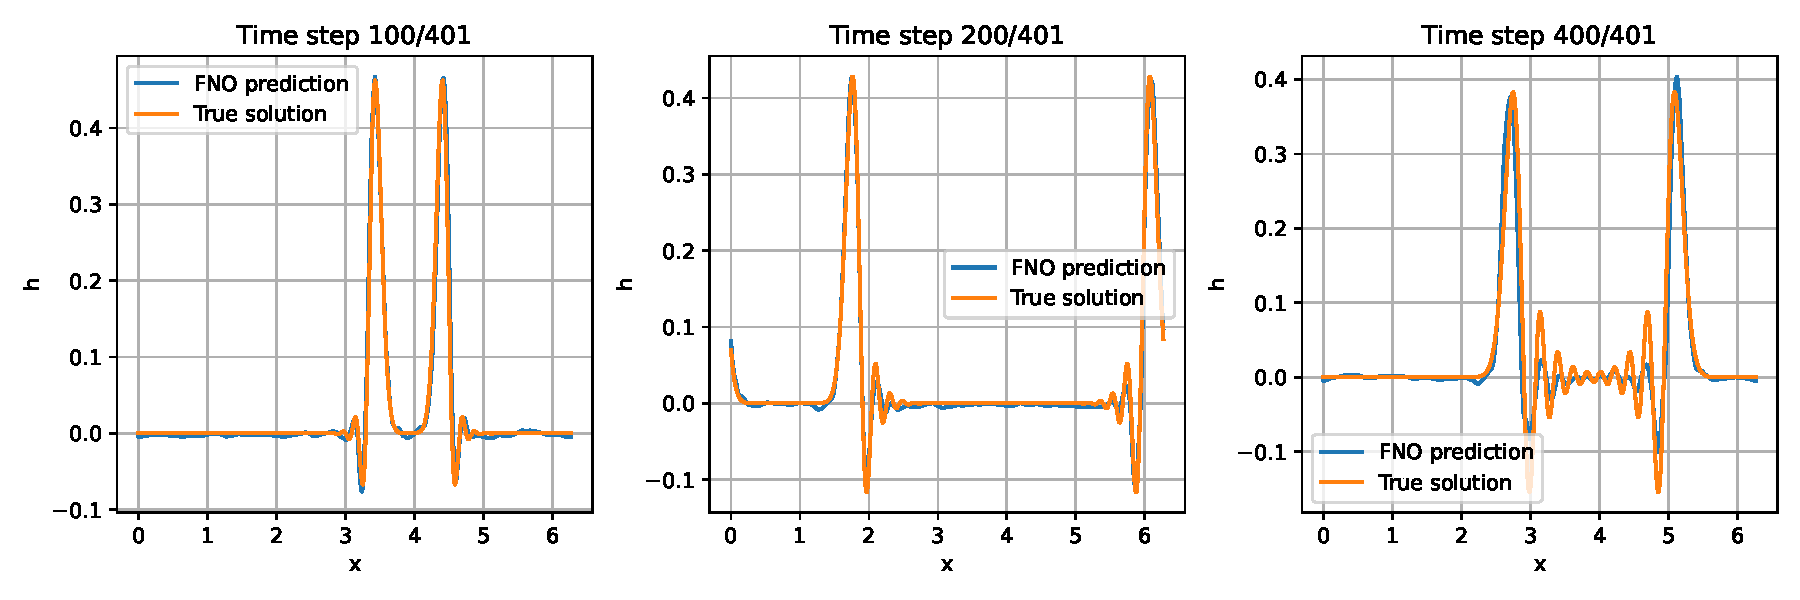
\includegraphics[width=\textwidth]{C:/Users/Matteo/Shallow-Water-Equations/plots/Spherical_linear_1D_FNO_timesteps_sigma=3.pdf}
    \caption{Results for the 1D SWE spherical CNN with sigma=1.}
\end{figure}





\section{FNO Toro test 1}
To test the FNO model on a more challenging problem, we consider the Toro test case 1.
We use the same model as before, but we train it on the data from the Toro test case 1.
Again, we use the first $80\%$ of the data for training and the last $20\%$ for testing.
The results of the model are shown in \autoref{fig:FNO_Toro_test1_predictions_3D} and \autoref{fig:FNO_Toro_test1_predictions}.

\begin{figure}[H]
    \centering
    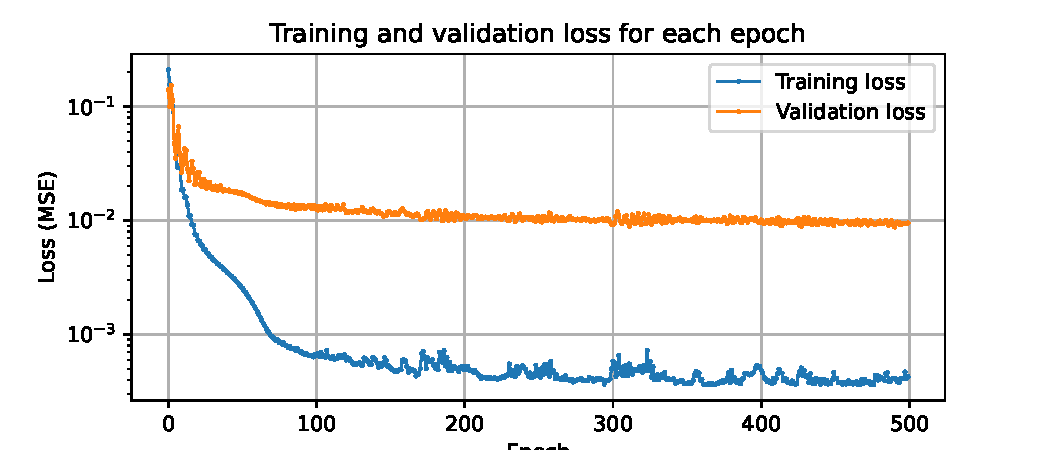
\includegraphics[width=0.7\textwidth]{C:/Users/Matteo/Shallow-Water-Equations/plots/torotest1_loss.pdf}
    \caption{FNO Toro test 1 loss.}\label{fig:FNO_Toro_test1_loss}
\end{figure}

\begin{figure}[H]
    \centering
    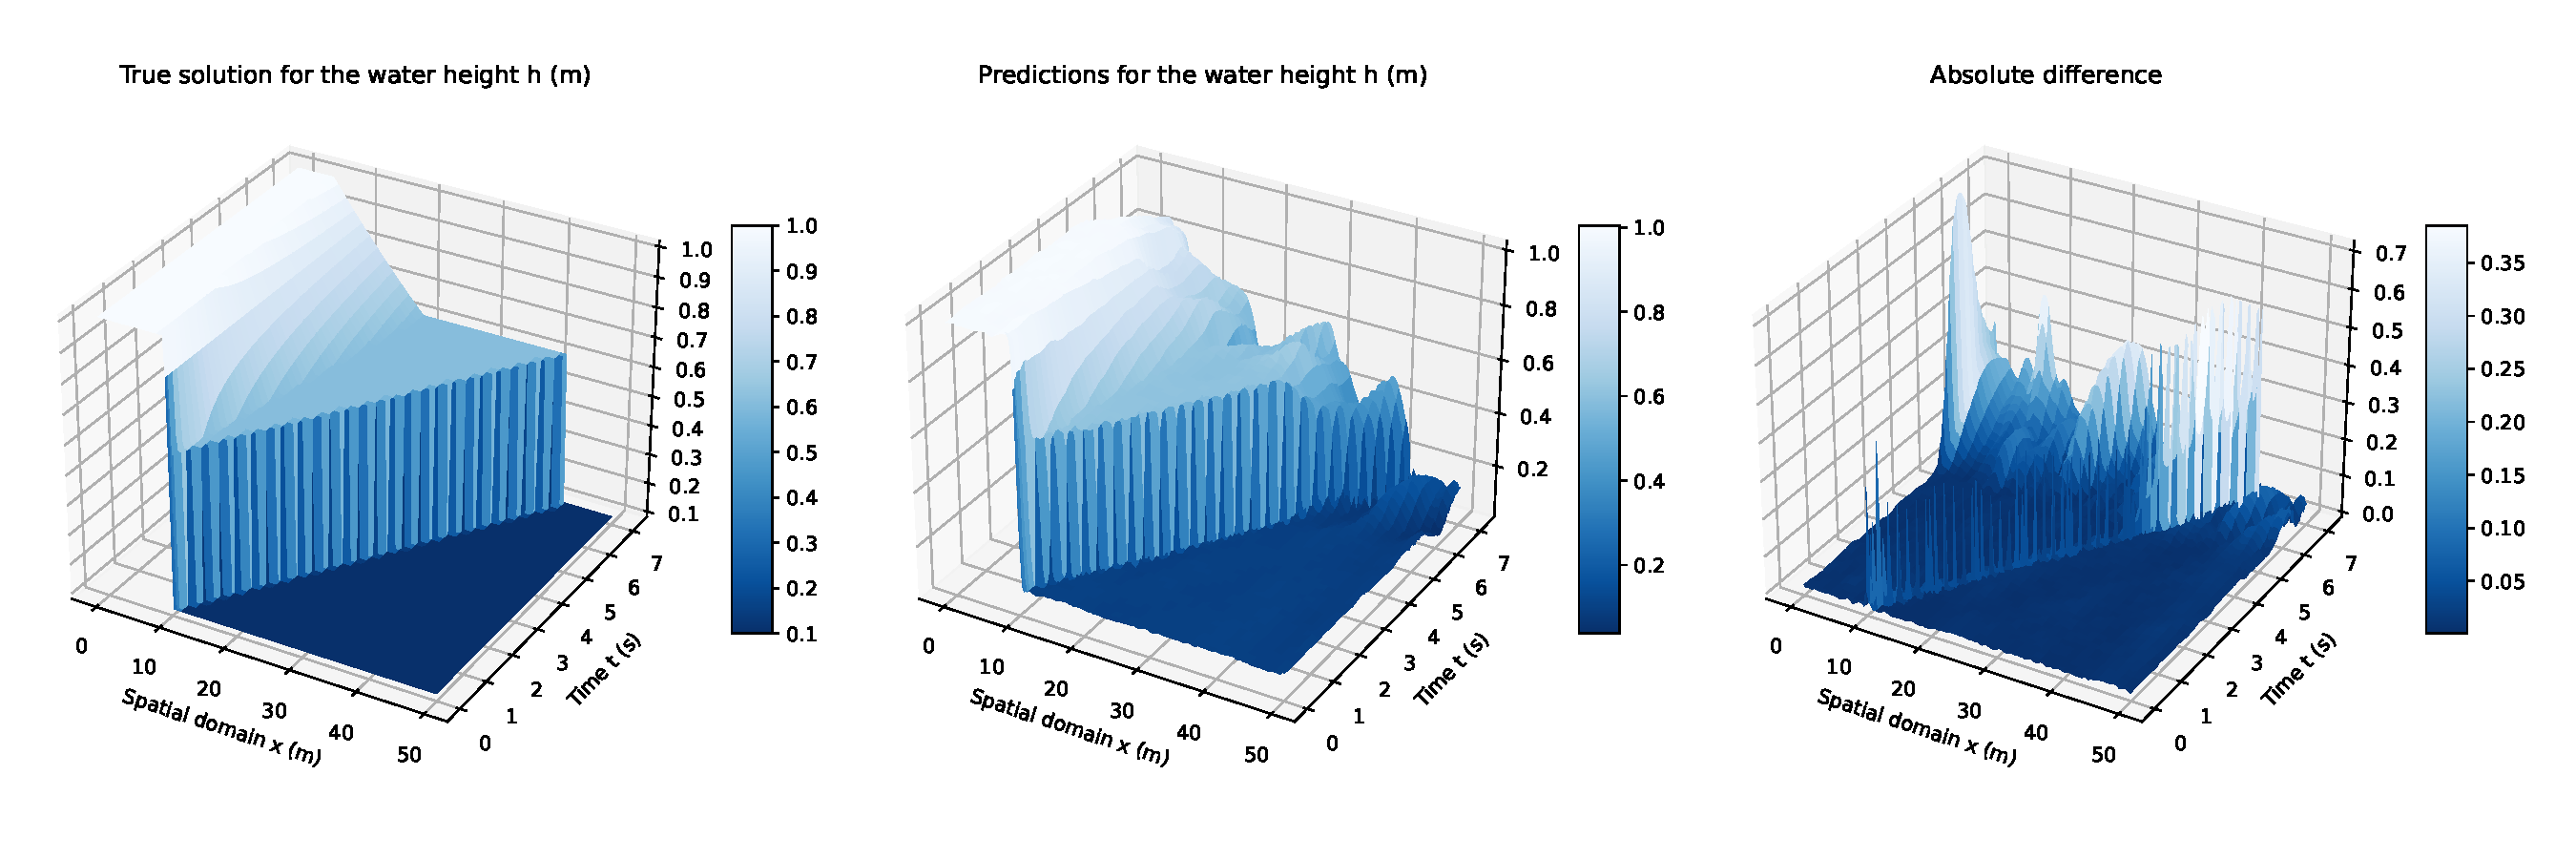
\includegraphics[width=0.9\textwidth]{C:/Users/Matteo/Shallow-Water-Equations/plots/torotest1_predictions_3D.pdf}
    \caption{FNO Toro test 1 predictions in 3d.}\label{fig:FNO_Toro_test1_predictions_3D}
\end{figure}


\begin{figure}[H]
    \centering
    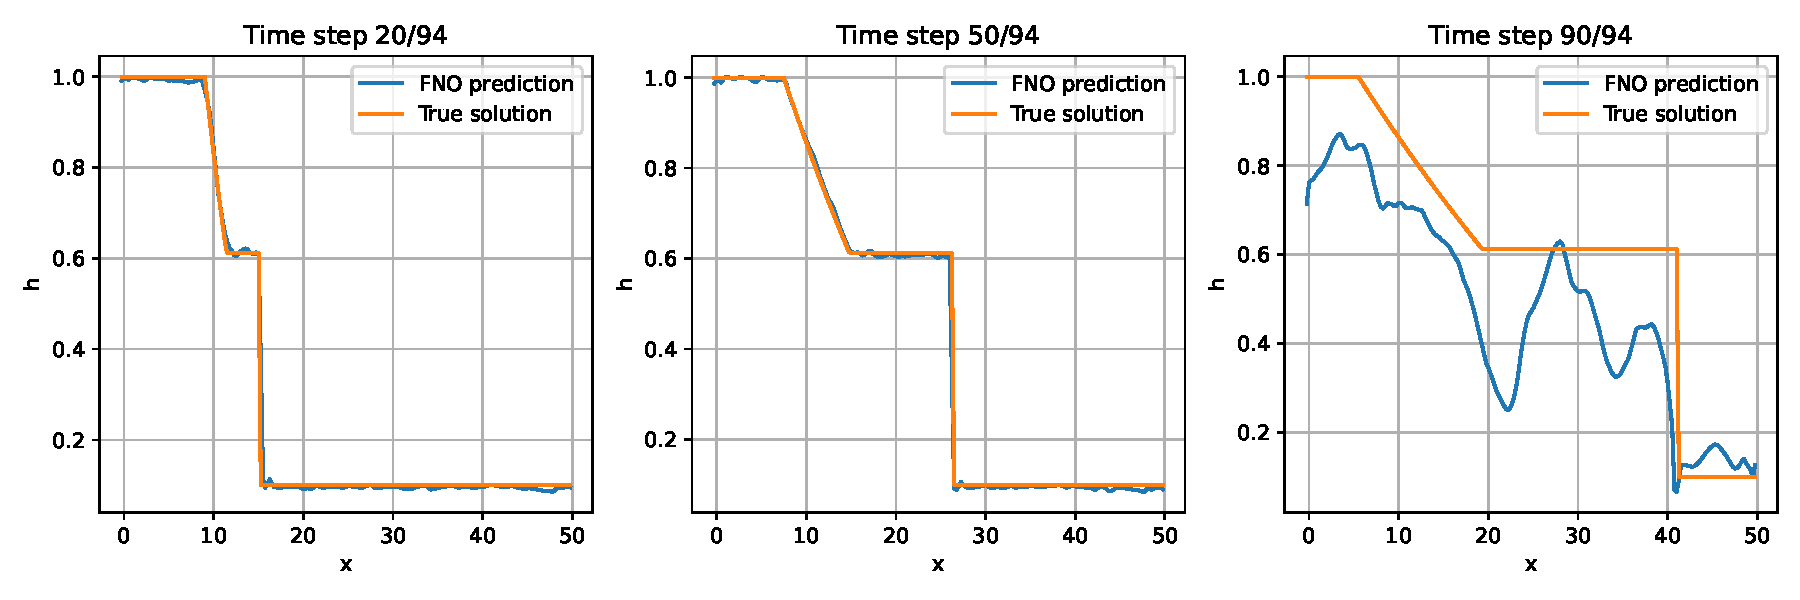
\includegraphics[width=0.9\textwidth]{C:/Users/Matteo/Shallow-Water-Equations/plots/torotest1_predictions_time_steps.pdf}
    \caption{FNO Toro test 1 predictions timesteps.}\label{fig:FNO_Toro_test1_predictions_time_steps}
\end{figure}


\begin{figure}[H]
    \centering
    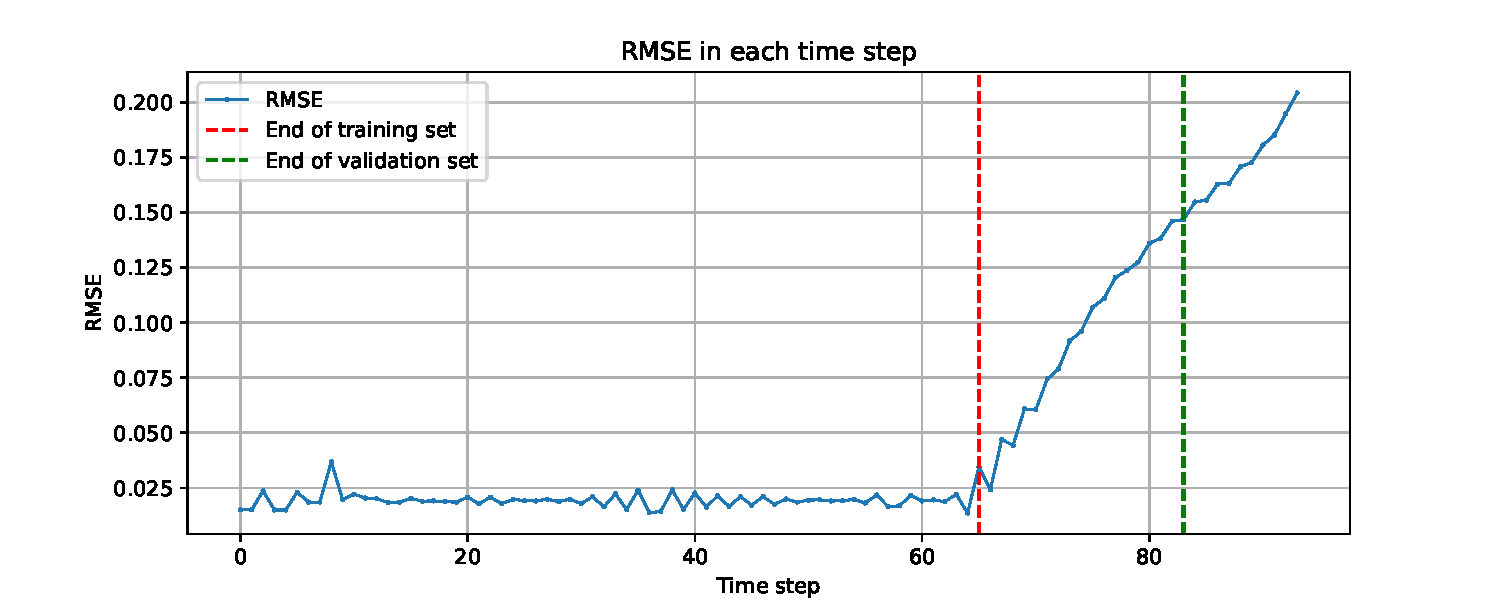
\includegraphics[width=0.7\textwidth]{C:/Users/Matteo/Shallow-Water-Equations/plots/torotest1_RMSE.pdf}
    \caption{FNO Toro test 1 predictions RMSE.}\label{fig:FNO_Toro_test1_rmse}
\end{figure}



\section{2D SWE long term prediction}
The results for the long-term predictions can be seen in \autoref{fig:2D_FNO_long_term_predictions}.
\begin{figure}[H]
    \centering
    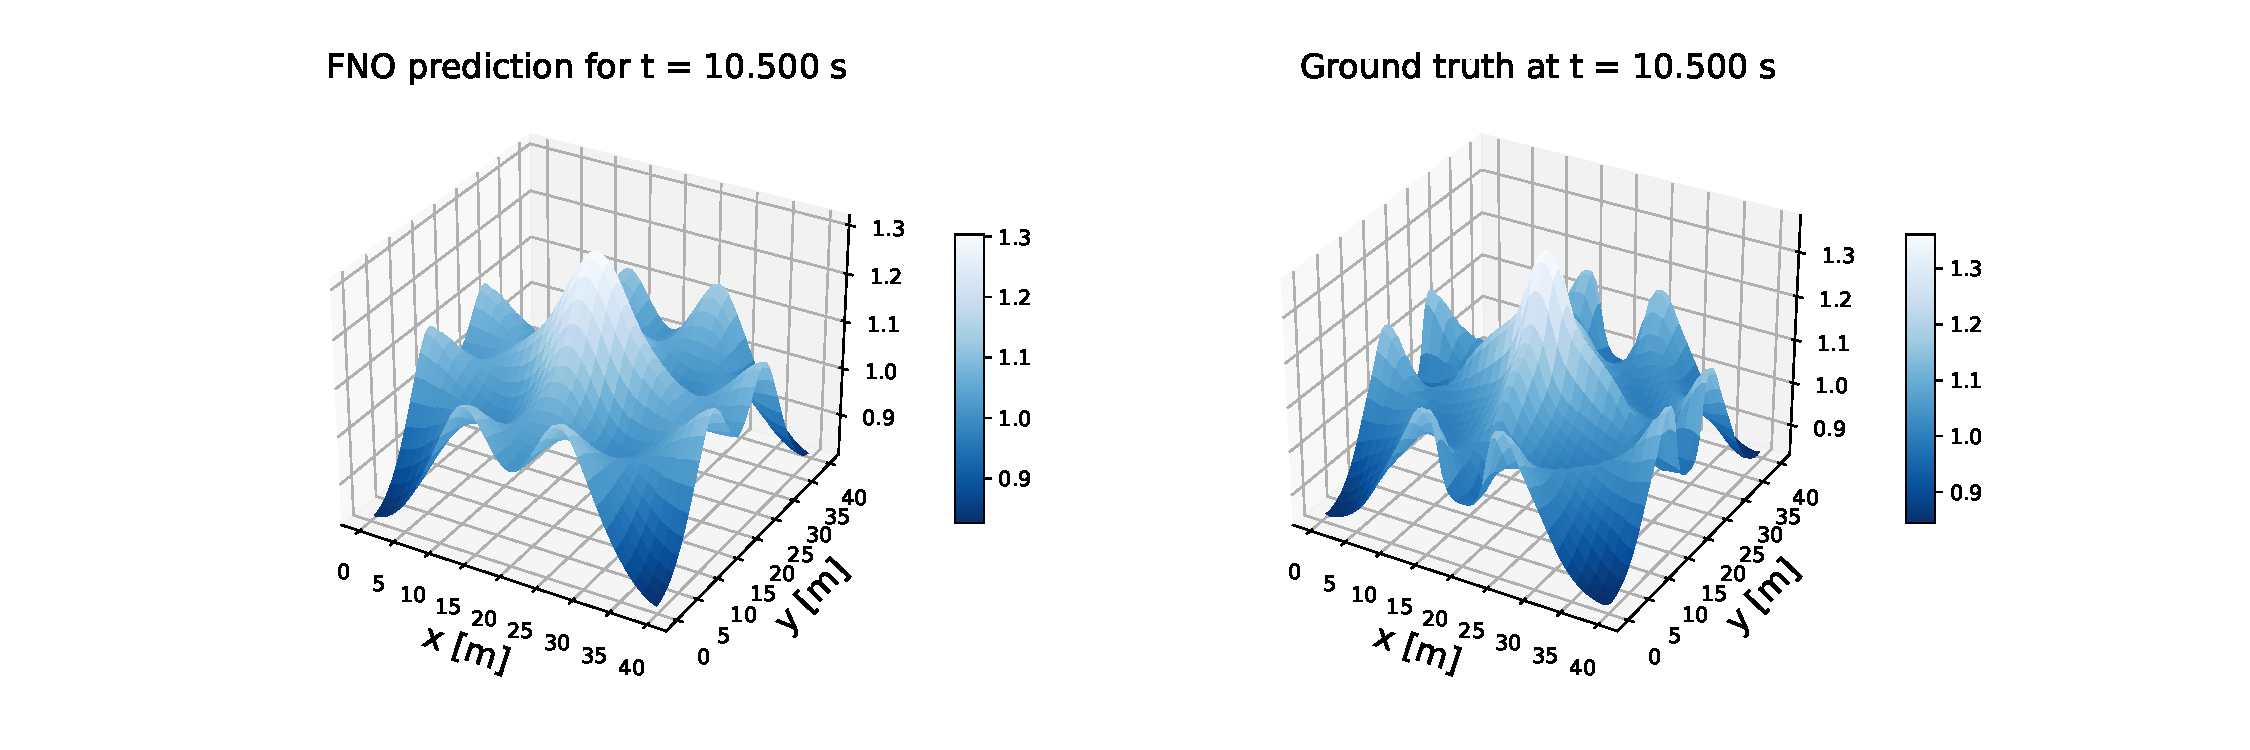
\includegraphics[width=\textwidth]{C:/Users/Matteo/Shallow-Water-Equations/plots/2D_FNO_long_term_predictions_Ntrain=64_Npred=64_idx=20.pdf}
    \caption{Long-term prediction for the 2D FNO model.}\label{fig:2D_FNO_long_term_predictions}
\end{figure}


\begin{figure}[H]
    \centering
    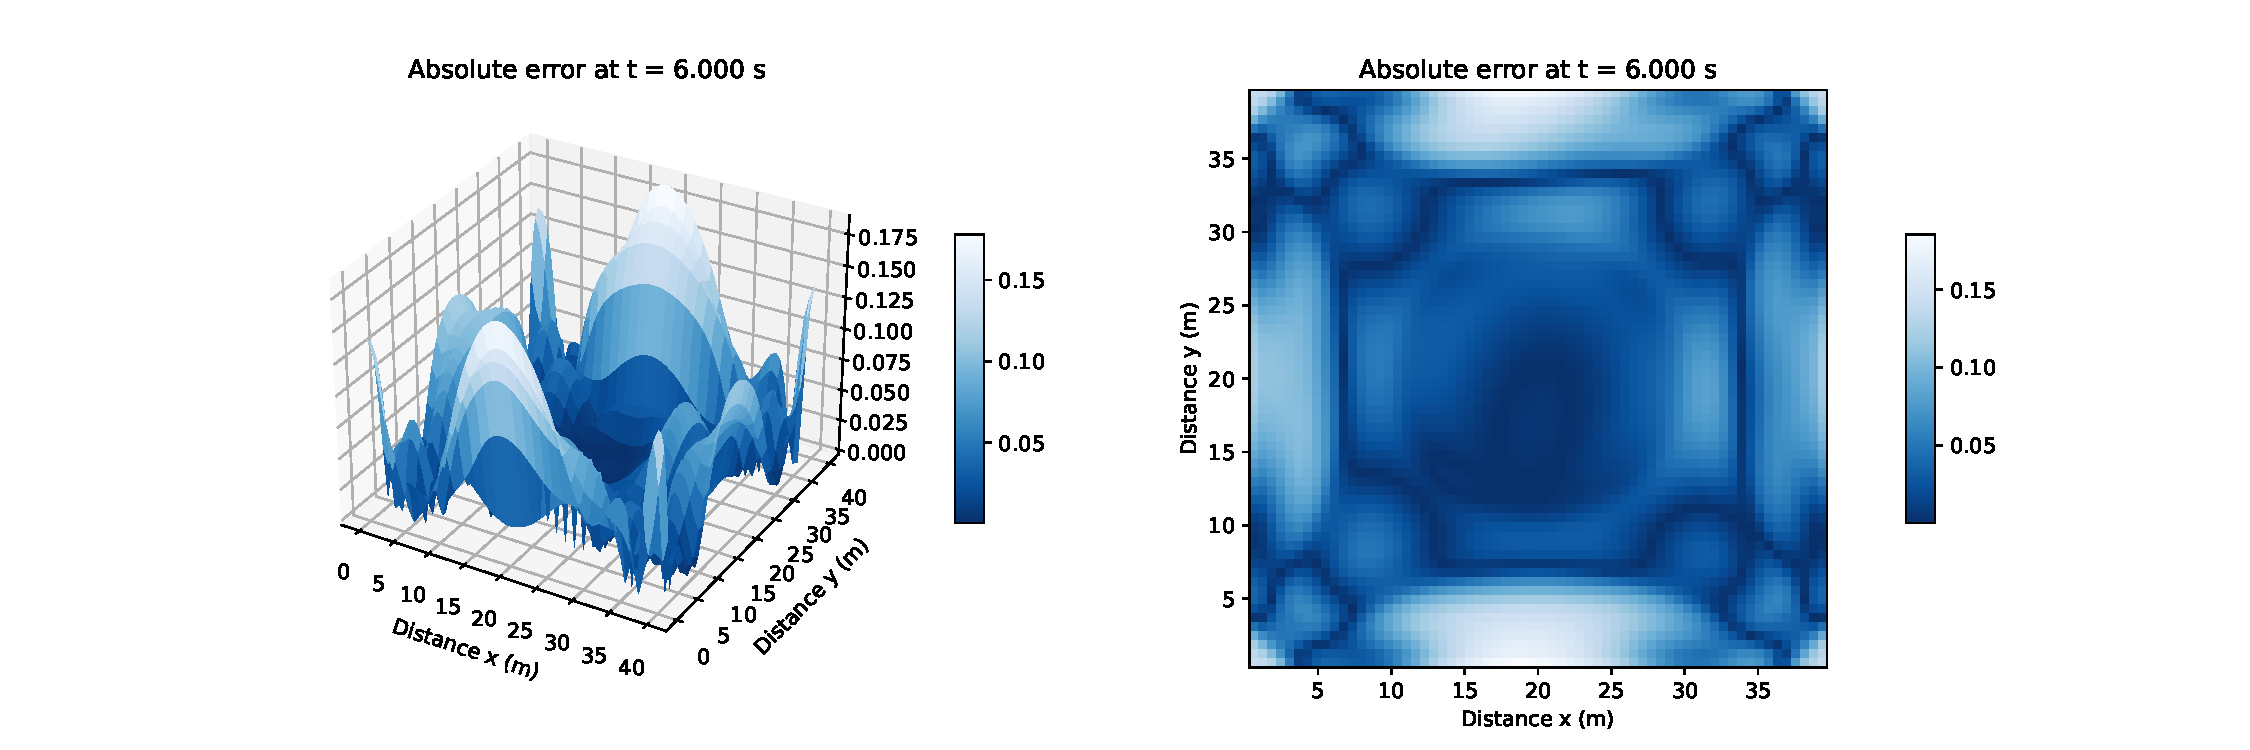
\includegraphics[width=\textwidth]{C:/Users/Matteo/Shallow-Water-Equations/plots/2D_FNO_long_term_predictions_error_Ntrain=64_Npred=64_idx=40.pdf}
    \caption{Error plot for the long-term prediction for the 2D FNO model.}\label{fig:2D_FNO_long_term_error_40}
\end{figure}




